% !TEX root = ../Main.tex
\chapter{平行关系}

"平行"在立体几何里\textbf{分三层}：线线平行、线面平行、面面平行。判定定理的共同主旨是——\textbf{把未知层的平行"降维"到已知层上，或"升维"到更高层中}。记住三张核心"判定图"，就掌握了所有平行问题的钥匙。

\section{线线平行的判定}

\state{线线平行的六种来源}{
    空间中两直线 $a \parallel b$ 的最常用判定：
    \begin{enumerate}
        \item[\textbf{(i)}] \textbf{公理 4（传递性）}：$a \parallel c, b \parallel c \implies a \parallel b$；
        \item[\textbf{(ii)}] \textbf{共面且无交点}：若 $a, b$ 在同一平面内且无公共点，则 $a \parallel b$；
        \item[\textbf{(iii)}] \textbf{面面平行的交线同向}：若 $\alpha \parallel \beta$，第三个平面 $\gamma$ 与两者分别交于 $a, b$，则 $a \parallel b$；
        \item[\textbf{(iv)}] \textbf{线面平行的性质定理}：若 $a \parallel \alpha$，过 $a$ 作平面 $\beta$，$\alpha \cap \beta = b$，则 $a \parallel b$；
        \item[\textbf{(v)}] \textbf{垂直于同一平面}：$a \perp \alpha, b \perp \alpha \implies a \parallel b$（第 3 章用）；
        \item[\textbf{(vi)}] \textbf{向量共线}：$\vec a \parallel \vec b$ 且不共点 $\implies a \parallel b$（向量法用）。
    \end{enumerate}
}

\section{线面平行的判定}

\state{线面平行判定定理}{
    \textbf{判定}：若 $a \parallel b$，$a \not\subset \alpha$，$b \subset \alpha$，则 $a \parallel \alpha$。

    用文字：\textbf{平面外一条直线，如果与平面内的一条直线平行，那么这条直线与此平面平行。}
}

\begin{center}
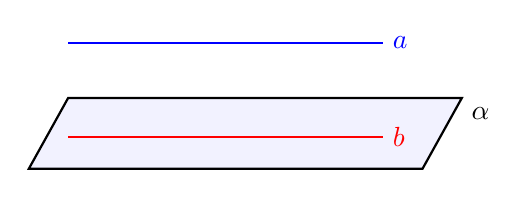
\begin{tikzpicture}[scale=1]
    \draw[thick, fill=blue!5] (-2.5, -0.4) -- (2.5, -0.4) -- (3, 0.5) -- (-2, 0.5) -- cycle;
    \draw[thick, red] (-2, 0) -- (2, 0);
    \node[red] at (2, 0) [right] {$b$};
    \draw[thick, blue] (-2, 1.2) -- (2, 1.2);
    \node[blue] at (2, 1.2) [right] {$a$};
    \node at (3, 0.3) [right] {$\alpha$};
\end{tikzpicture}
\end{center}

\state{线面平行的三种来源}{
    证 $a \parallel \alpha$ 的常用路径：
    \begin{itemize}
        \item[\textbf{(i)}] \textbf{找面内一平行线}——在 $\alpha$ 内找到 $b$ 使 $a \parallel b$（最常见）；
        \item[\textbf{(ii)}] \textbf{面面平行反推}——若 $a \subset \beta$ 且 $\beta \parallel \alpha$，则 $a \parallel \alpha$；
        \item[\textbf{(iii)}] \textbf{向量与法向量垂直}——$\vec a \cdot \vec n_\alpha = 0$ 且 $a$ 不在 $\alpha$ 内。
    \end{itemize}
}

\state{线面平行的性质定理}{
    \textbf{性质}：若 $a \parallel \alpha$，过 $a$ 作平面 $\beta$，$\alpha \cap \beta = b$，则 $a \parallel b$。

    用文字：\textbf{一条直线与一个平面平行，过这条直线的任一平面与此平面的交线，都与这条直线平行。}
}

\section{面面平行的判定}

\state{面面平行判定定理}{
    \textbf{判定}：若 $\alpha$ 内两条相交直线 $a, b$ 都与 $\beta$ 平行，则 $\alpha \parallel \beta$。

    用文字：\textbf{如果一个平面内的两条相交直线都与另一个平面平行，那么这两个平面平行。}

    \textbf{注意}：两直线\textbf{相交}是关键——两条平行直线\textbf{不够用}（反例：两平行线都与交线平行，但两平面却相交）。
}

\begin{center}
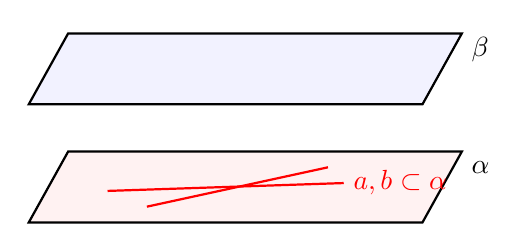
\begin{tikzpicture}[scale=1]
    \draw[thick, fill=blue!5] (-2.5, 1.1) -- (2.5, 1.1) -- (3, 2) -- (-2, 2) -- cycle;
    \draw[thick, fill=red!5] (-2.5, -0.4) -- (2.5, -0.4) -- (3, 0.5) -- (-2, 0.5) -- cycle;
    \draw[thick, red] (-1.5, 0) -- (1.5, 0.1);
    \draw[thick, red] (-1, -0.2) -- (1.3, 0.3);
    \node[red] at (1.5, 0.1) [right] {$a, b \subset \alpha$};
    \node at (3, 1.8) [right] {$\beta$};
    \node at (3, 0.3) [right] {$\alpha$};
\end{tikzpicture}
\end{center}

\state{面面平行的性质定理}{
    \textbf{性质}：若 $\alpha \parallel \beta$，$\gamma \cap \alpha = a$，$\gamma \cap \beta = b$，则 $a \parallel b$。

    用文字：\textbf{两平面平行，第三个平面与它们的交线平行。}
}

\rmkb{
    \textbf{平行判定"金三角"}：
    \begin{center}
    \begin{tikzpicture}[scale=1.0]
        \node (l) at (0, 1.2) {\textbf{线线平行}};
        \node (p) at (-2, -0.5) {\textbf{线面平行}};
        \node (pp) at (2, -0.5) {\textbf{面面平行}};
        \draw[<->, thick] (l) -- (p) node[midway, above left] {\small 判定/性质};
        \draw[<->, thick] (l) -- (pp) node[midway, above right] {\small 交线};
        \draw[<->, thick] (p) -- (pp) node[midway, below] {\small 两相交线}
        ;
    \end{tikzpicture}
    \end{center}

    \textbf{做题套路}：要证的目标在"高层"时（如面面平行），\textbf{往下降维}（找两条相交线 \& 它们的线面平行）；要证的目标在"低层"时（如线线平行），\textbf{往上升维}（升到线面、面面平行，再用性质定理反推）。
}
